%% LyX 2.2.3 created this file.  For more info, see http://www.lyx.org/.
%% Do not edit unless you really know what you are doing.
\documentclass{article}
\usepackage[T1]{fontenc}
\usepackage[utf8]{inputenc}
\usepackage{kotex}
\usepackage{verbatim}
\usepackage{booktabs}
\usepackage{graphicx}
\usepackage[unicode=true,
 bookmarks=false,
 breaklinks=false,pdfborder={0 0 1},colorlinks=false]
 {hyperref}
\usepackage{breakurl}

\makeatletter

%%%%%%%%%%%%%%%%%%%%%%%%%%%%%% LyX specific LaTeX commands.
%% Because html converters don't know tabularnewline
\providecommand{\tabularnewline}{\\}

%%%%%%%%%%%%%%%%%%%%%%%%%%%%%% User specified LaTeX commands.


% if you need to pass options to natbib, use, e.g.:
% \PassOptionsToPackage{numbers, compress}{natbib}
% before loading nips_2017
%
% to avoid loading the natbib package, add option nonatbib:
% \usepackage[nonatbib]{nips_2017}

\usepackage[final]{nips_2017}


% to compile a camera-ready version, add the [final] option, e.g.:
% \usepackage[final]{nips_2017}

% allow utf-8 input
% use 8-bit T1 fonts
% hyperlinks
\usepackage{url}% simple URL typesetting
% professional-quality tables
\usepackage{amsfonts}% blackboard math symbols
\usepackage{nicefrac}% compact symbols for 1/2, etc.
\usepackage{microtype}% microtypography

\title{President Sings - Voice Conversion Using Generative Adversarial Network}

% The \author macro works with any number of authors. There are two
% commands used to separate the names and addresses of multiple
% authors: \And and \AND.
%
% Using \And between authors leaves it to LaTeX to determine where to
% break the lines. Using \AND forces a line break at that point. So,
% if LaTeX puts 3 of 4 authors names on the first line, and the last
% on the second line, try using \AND instead of \And before the third
% author name.

\author{
  Chang Minwook\\
  2014210066\\
  Department of Computer Science\\
  Korea University\\
  \texttt{fromme0528@gmail.com} \\
  %% examples of more authors
  \And
  Cho Youngwoo\\
  2014210085\\
  Department of Computer Science\\
  Korea University\\
  \texttt{cyw314@gmail.com} \\
  \AND
  Min Jungki\\
  2014210093\\
  Department of Computer Science\\
  Korea University\\
  \texttt{eternalray123@gmail.com} \\
  %%\And
  %%Goyangii\\
  %%2014210000\\
  %5Family of Felidae\\
  %%\texttt{ya-ong@cuteness.com} \\
  %% \And
  %% Coauthor \\
  %% Affiliation \\
  %% Address \\
  %% \texttt{email} \\
}

\@ifundefined{showcaptionsetup}{}{%
 \PassOptionsToPackage{caption=false}{subfig}}
\usepackage{subfig}
\makeatother

\begin{document}
% \nipsfinalcopy is no longer used

\maketitle
\begin{abstract}
Our project aims to synthesize someone's voice singing a song, using Generative Adversarial Network(cite) in short, GAN.
There is an ongoing research about speech synthesis. The majority of the work have been done in the area of Text-to-Speech(TTS)(cite) where it takes text as an input and produces speech as an output. The limitation of TTS we think is that even though it is posssible to reproduce someone's voice, it is hard to capture the features that are the key components in singing such as voice tone, voice pitch, and voice tempo.It is hard to put those voice features in TTS model as an input, as well as make model to learn those features. Another difficulty is that we can't simply earn such feature-labled data.
The data we use to learn our model is unpaired data. It is very infeasible to get the data of Trump's singing voice or the data of speaking exactly the same thing that Trump says.
Cycle-GAN, current state-of-art GAN, make it possible to convert between unpaired data. Thus we use Cycle-GAN's approach in our voice conversion model. 


\end{abstract}

\section{Project Overview}

A few months ago, a video titled "Barack Obama Singing Shape of You" had been uploaded on Youtube\footnote{\href{https://www.youtube.com/watch?v=bmhbqKT7ONo}{https://www.youtube.com/watch?v=bmhbqKT7ONo}}. Not that Obama actually sang the song, the editor who uploaded the video collected Obama's speech videos and stitched them so that it looks like as if Obama sang the song. This is just one example of funny Internet meme: uploading videos of famous songs sung by celebrities' voice. Although watching those edited videos is fun, the editor has to put a lot of time and effort to make one such video. First, the editor needs plenty of videos that contain voice that she wants to synthesize. Collecting these videos may take a few weeks or worse, a few months. Second, the editor has to edit videos "manually", which means she has to find a time frame of a video that captures the voice needed to build up the song. Then she extracts those time frames, stitchs them, and finally makes one funny piece of music. We think this process, though the result is cool, is definitely painful and inefficient. Here, our project aims to synthesize someone's voice singing a song, using Generative Adversarial Network\cite{Goodfellow:2014td} in short, GAN.

There is an ongoing research about speech synthesis. The majority of the work have been done in the area of Text-to-Speech(TTS)\cite{Allen:1987td} where it takes text as an input and produces speech as an output. The limitation of TTS we think is that even though it is posssible to reproduce someone's voice, it is hard to capture the features that are the key components in singing such as voice tone, voice pitch, and voice tempo. In TTS, the model learns the matching between each phoneme and target voice with a certain feature combination, while in singing a song, same phonemes may have different voice features. Thus, we plan to design our model as Speech-to-Speech(STS), where it takes speech as an input and produces speech as an output. Although this approach is uncommon, we try to build STS model using GAN.

To train our model, large amounts of voice data(perhaps 2\textasciitilde10 hours) have to be collected. These voice data, whether they are target voice or not is not matter because we both have to collect true label data and false label data. We then preprocess the sound data to make a training set because dealing with raw sound data is complicated thing. We used Short-Time Fourier Transformation(STFT)\cite{Jont:1977td} to preprocess the data. Our model, has three internal models. One is Autoencoder, which makes latent vector for the audio. Next one is Generator model, which takes our preprocessed data as an input and produces target voice as an output. Last one is Discriminator model, which takes voice data as an input and outputs true, if the input resembles the target voice, or false, if the input does not sound like the target voice.
   
Our novel technique can be utilizied in converting voice of celebrities who are alive and also who passed away, so that the fan of those celebrities can enjoy their voice singing new, contemporary songs even after they are dead.

Before beginning our project, we have two major concerns. One is that what if we cannot sufficiently extract the features that consist of singing voice. If we cannot extract the features well enough, the quality of the output will be poor and the output will not resemble the target voice. The other is that our technique can be manipulated by those who want to break the biometric voice authentication system\cite{Vallabhu:2012td}. Biometric voice authentication system uses a client's voice to authenticate whether the given voice is vaild. Although it is not common to use voice recognition technique in traditional authentication area, if that kind of voice authentication applications prevail in the near future, the chance for the intentional attacker to maliciously exploit our technique to break in those applications also goes up.

For our future work, we can think of the way to input the voice singing a song without removing MR. We can consider MR as sort of noise and if we make the model resilient enough to the noise(which is MR in this case). We can develop the noise-resilience model which can directly produce the target voice with MR.

\section{Data Sets}

We collected audio data on Youtube and SLR\cite{SLR:2015td} data sets. and we preprocess those data to make 10 hours spectrogram. We cut the audio data into three seconds time frame and do STFT that frame. Here the sampling rate is 51200Hz, and the channel is mono. With STFT configuration we followed Praat\cite{Praat:2017td}, n\textunderscore fft to 2048, hop\textunderscore length to 256, window\textunderscore length to 1024.

We normalized our spectrogram. To reflect sparseness, we calculate the mean and variance of data larger than 1. Here we appied idea of multiplying 2 to variance\cite{Kaiming:2015td}

We didn't use dB scale. This is because dB scale is log scale, which is more sensitive. In our case, the noise is a big problem, and the log scale makes this noise problem much more complicated.

\section{Problem Definition}

Our goal is to transform input voice into target voice we want. This kind of problem is often called "many to one voice conversion".\cite{Lifa:2016td} In general, voice that voice conversion deals with is talking voice, but in our case we want to deal with singing voice. This is the reason why we don't use TTS. Current TTS (ex)Tacotron, Deep Voice) can synthesize target voice. But that doesn't mean that we can transform input voice to make target voice sing. Because in singing, voice features such as pitch, tempo are important components. It is hard to put those voice features in TTS model as an input, as well as make model to learn those features. Another difficulty is that we can't simply earn such feature-labled data.

\section{Background}

Before we propose our model, we illustrate background about voice conversion.

\subsection{Spectrogram}

Music files in computer represent waveform with respect to amplitude or power. Neither human nor machine learning model can easily recognize this representation and find musical features. Therefore, we transform music wave into spectrogram to help model understand better. 

Spectrogram is a graph that represents energy of given signal with respect to time and frequency. Spectrogram is generated using Short-Time Fourier Transformation(STFT). STFT does Fast Fourier Transformation(FFT) given signal with very small window length and hop length, which is used to slide a little bit. The result of STFT is matrix of complex numbers. In general, magnitude of those complex numbers are used in analysis or machine learning.

Our model also uses magnitude of complex numbers. In this case, the phase information is lost, so we can't reconstruct audio signal from magnitude. So we use Griffin-Lim algorithm\cite{Daniel:1984td} to iteratively find the lost phase information and reconstruct original audio signal given magnitude of spectrogram.

\subsection{Voice Feature}

We assume that in spectrogram, we can extract voice features(pitch, tempo, formant, intonation ...)

Especially, the pronounciation of vowel is represented by formant in spectrogram. Formant is a band parallel to time axis in spectrogram. The difference between the first formant in lowest frequency and the second formant in next lowest frequency tells that the given audio frame represents which vowel. In case of consonant, a band parallel to frequency axis in spectrogram represents consonant information.

Pitch is represented by frequency. difference between interval and pitch is that interval is the relative difference while pitch is the absoulte value represented by hertz(Hz). Same pronounciation with different pitch represented by the parallel transference of formant with respect to frequency axis. Intonation is change of pitch.

Tone is determined by spectrum and envelope. Envelope is change of waveform during sound exists. Voice is compound sound mixed with many different frequencies. Spectrum represents the ratio of these frequencies.

\section{Model Idea}

In voice conversion, the key point is that how to convert intonation and tone while keeping pitch, tempo, and pronounciation. We consider this as a two viewpoint. First, Style Transfer of spectrogram image. Given a spectrogram image, we convert it into spectrogram that has target's style.

Secondly, we think of it as a change of probability distribution. If we see a window of spectrogram, we can see that it is a 2D graph with respect to frequency and amplitude. The graph is a combination of Gaussian probability distributions that has formant as a mean and voice features as a variance. So our model can learn these mean and variance
to convert a input probability distribution to target probability distribution.

In general voice conversion models, they use time-dependent model such as RNN. We think we can reflect those two ideas without using RNN, with only using CNN. In phonetics, there are basic sound called IPA. We can classify every single language in the world based on this IPA. This means if we well define convolution filter, we can capture all the features in the voice.

The data we use to learn our model is unpaired data. It is very infeasible to get the data of Trump's singing voice or the data of speaking exactly the same thing that Trump says.
Cycle-GAN, current state-of-art GAN, make it possible to convert between unpaired data. Thus we use Cycle-GAN's approach in our voice conversion model. 

In Cycle-GAN, it assumes that it can reconstruct the converted data. But in our case, this is a bit awkward because this means that we have to reconstruct random voice from Trump's voice, which is constructed from again, random voice. In order to handle this awkwardness and consider cycle loss, we introduce autoencoder\cite{Deng:2010td} to make latent vector and use it as an input to our GAN model.

\section{Model Structure}

MODEL STRUCTURE

Our model has three parts, autoencoder, generator, and discriminator.

\subsection{Autoencoder}

Current structure of autoencoder is very simple. We have encoder and decoder to make result have same shape with input.

Structure of the encoder(denoted by Enc) is as follows.

Conv(3*3, stride 1, 16ch) – batchnorm – relu – conv(5*5, stride3, 32ch) – batchnorm relu – conv(1*1, stride1, 1ch)

Structure of the decoder(denoted by DecR) is as follows.

Deconv(5*5, stride3, 32ch) – batchnorm – relu or leakyrelu 0.05 – deconv(3*3, stride1, 16ch) – batchnorm – relu or leakyrelu 0.05 - deconv(1*1, stride1, 1ch)

The latent vector between encoder and decoder is not like the normal latent vector, which has information that is hard to recognize, it is more like the activation map in convolution.

Learning of autoencoder utilize pixelwise L1 loss with respect to input spectrogram x and output spectrogram xR,

\[L_{reconstuction} (Enc,DecR,x) = \mid\mid x-xR \mid\mid_1 = \mid\mid x-DecR(Enc(x)) \mid\mid_1\]

and make this loss minimize.

\subsection{Generator}

Our generator, DecT is same as decoder in autoencoder with different weight. This is because decoder solves harder problem than generator does. DecR has to reconstruct spectrogram that is same as input spectrogram, while generator only needs to reconstruct spectrogram that represents target voice. This means the range of decoder is larger than the range of generator. Thus if our decoder can reconstruct the given input spectrogram, our generator can generate a spectrogram of target voice.

In the meantime, a spectrogram generated by generator can be an unrecognizable by human. That means the voice features are not in the spectrogram. So we need loss function between latent vector of given input spectrogram and the latent vector of generated spectrogram by generator. This is the reason why we introduce the cycle loss,

\[L_{cycle} (Enc,DecT,x) = \mid\mid Enc(x)-Enc(DecT(Enc(x))) \mid\mid_1\]

\subsection{Discriminator}

In our model, discriminator does two things. First, like the normal GANs, discriminator judges whether the input is real or fake. Second, discriminator judges whether the input spectrogram is target voice or not. We don't have the labled data of target voice so we add this condition to make generator generate target voice. We followed the discriminator model from these.(two papers) Discriminator works as follows.

conv(11*11, stride4, 96ch) – batchnorm – relu – maxpool(2) – conv(5*5, stride1, 256ch) – batchnorm – relu – maxpool(2) – conv(3*3, stride1, 386ch) – batchnorm – relu – maxpool – conv(3*3, stride1, 256ch) – batchnorm – relu – maxpool – fc(4096) – relu – fc(2) – sigmoid

Output is 2D vector, first column means whether the input spectrogram is real or generated from the generator, second column means whether the input spectrogram represents Trump's voice or not. We calculate cross entropy loss as follows.

\[L_{discriminator} (Enc,DecT,Dis,x,y)= H(Dis(DecT(Enc(x))))[0],0)+H(Dis(x)[0],1)+H(Dis(x)[1],y)\]

Here, we don't use second column loss from the generated spectrogram because it is not helpful in the early phase of learning and it can generate totally wrong gradient.

\section{Result}

In out project we want to do something new, we made our model as simple as possible to know whether it is possible approach or not.

Current model can only reconstruct the given input spectrogram. The reason that the voice conversion is not working is that somehow our discriminator cannot discriminate the target voice. We followed exactly the same discriminator structure in the papers\cite{Ossama:2014td}\cite{Lior:2015td}. We estimate this is because the configuration of our spectrogram and theirs is different.

Also, the noise is a big problem. The reason noise happens is that in original spectrogram, there are zero values that represents empty sound, but in our reconstructed spectrogram, there are no zero values, only near-zero values, which makes noise.

\section{Evaluation}

In training phase, we proceed with 12288 spectrogram, learning rate of 1e-4, 10 epcoch and batch size of 32. The number of Trump's voice spectrogram is around 2200. We cut front and back part of the audio a little bit to make sure there is no empty sound. 

Currently, conversion is not working properly and we can't define ground truth exactly, we couldn't conduct exact experiment. Instead, we focused on loss. Below are the graphs of loss for three cases.

\begin{figure}[!htb]
  \minipage{0.32\textwidth}
  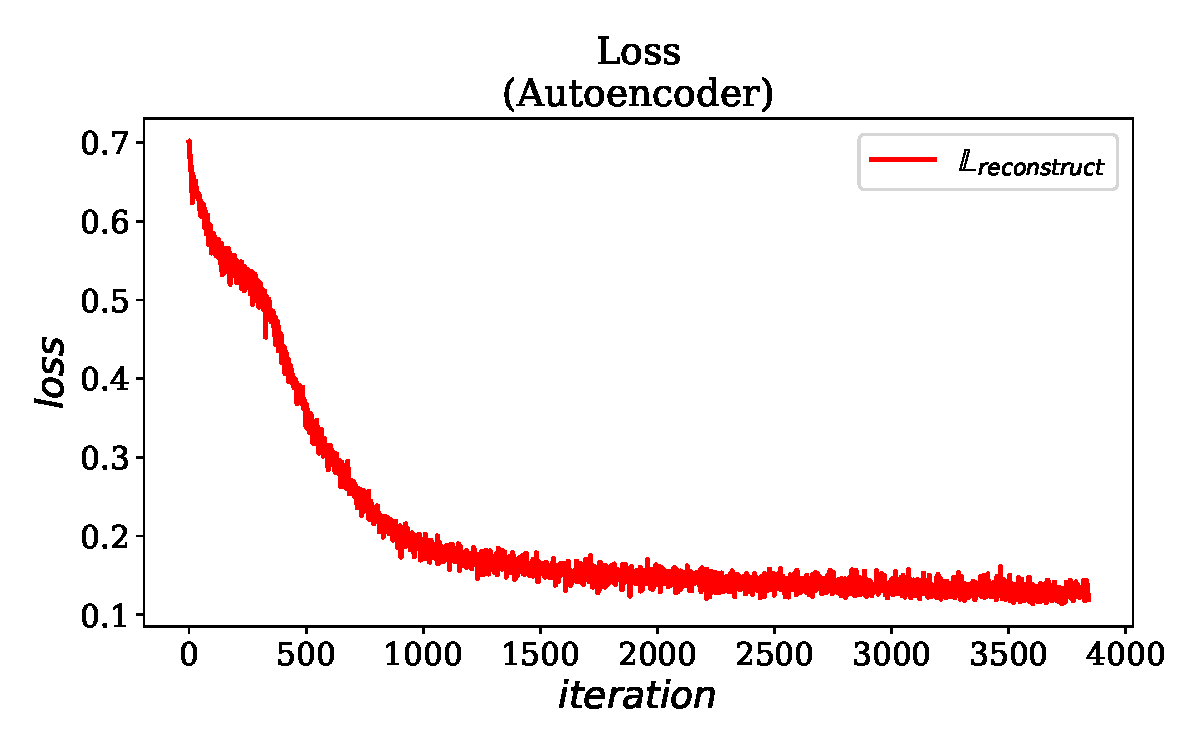
\includegraphics[width=\linewidth]{loss_graph/ae_loss_plot}
  \caption{autoencoder loss}
  \endminipage\hfill
  \minipage{0.32\textwidth}
  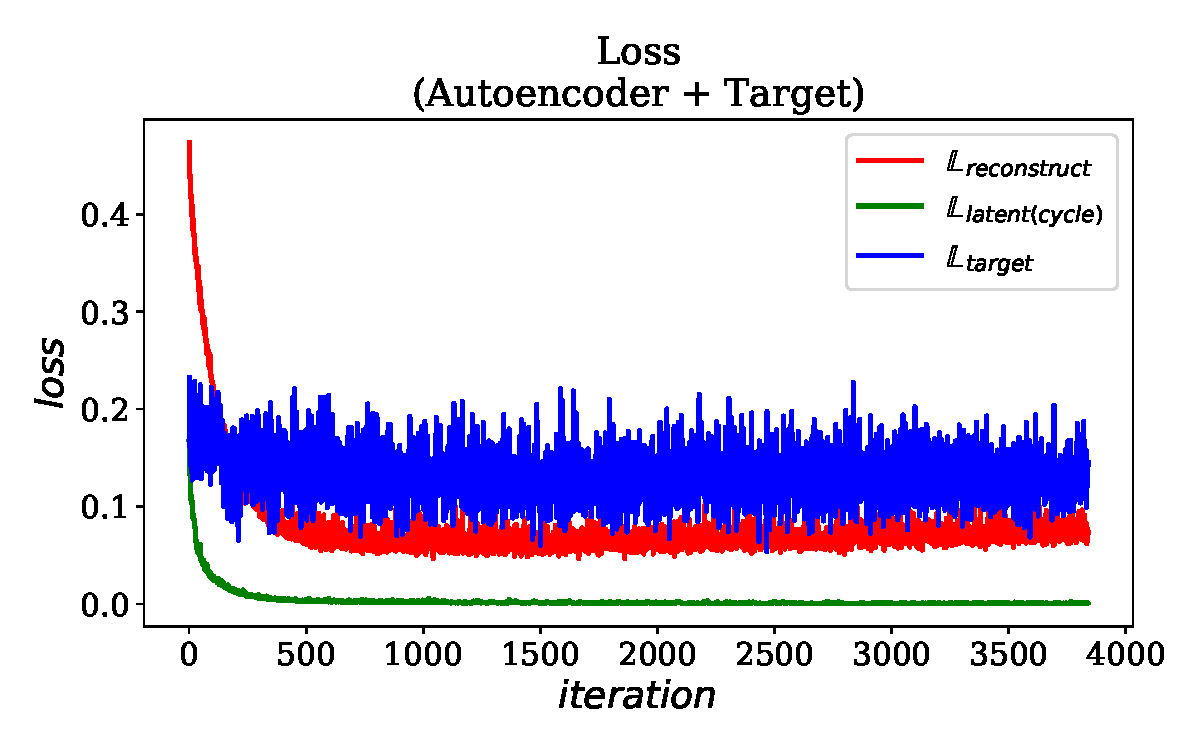
\includegraphics[width=\linewidth]{loss_graph/ae_target_loss_plot}
  \caption{autoencoder + target}
  \endminipage\hfill  
  \minipage{0.32\textwidth}
  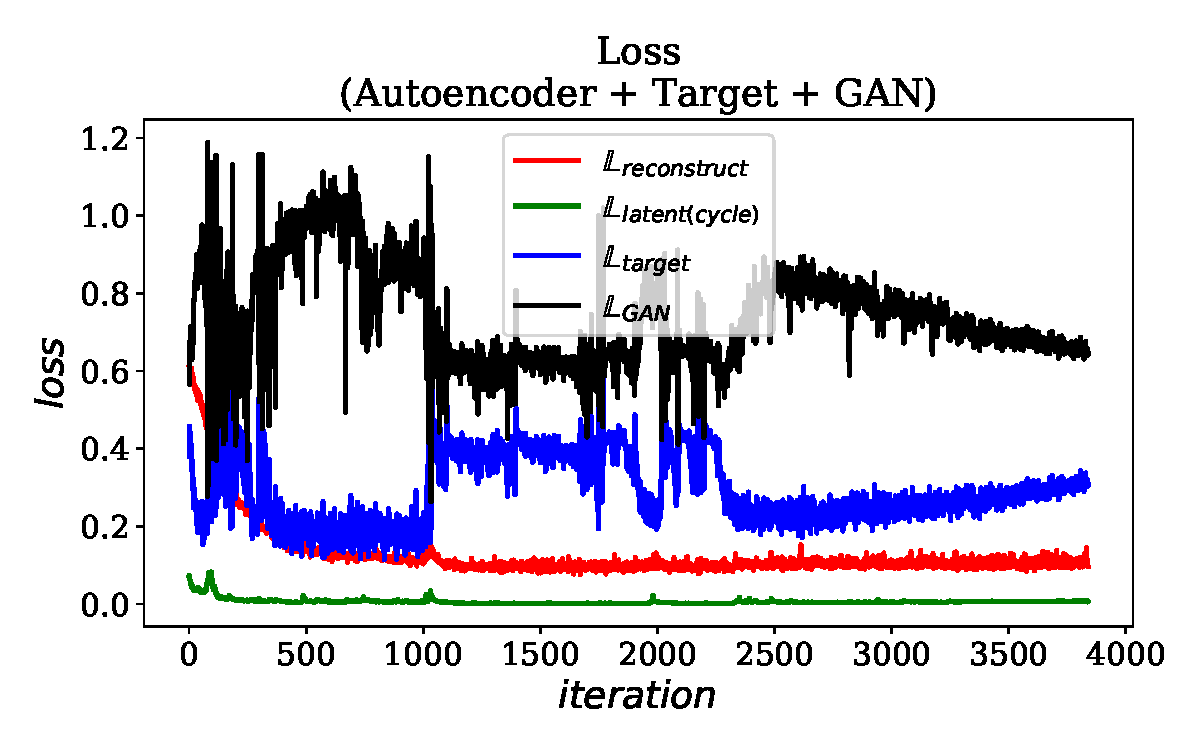
\includegraphics[width=\linewidth]{loss_graph/ae_target_gan_loss_plot}
  \caption{AE + target + GAN}
  \endminipage\hfill
\end{figure}

Autoencoder's reconstruction loss and latent vector's cycle loss diminished well, but loss of discriminator heavily fluctuated. This is the reason voice conversion failed.

Also, autoencoder's loss did not converge perfectly, so if we increased epoch, the loss may have decreased more.

For the spectrogram, we chose 3 audio, one is speech without background music, next one is humming with small background music, last one is singing song with loud background music. If we look these spectrograms, we can see that the capability of model to reconstruct and change the target audio, as well as tell apart background music and voice sound. We used Praat to plot the spectrograms and the result of FFT.

\subsection{Autoencoder}

\begin{figure}[!htb]
  \minipage{0.5\textwidth}
  \includegraphics[width=\linewidth]{figures/ae_loss/spectro_original_speech}
  \caption{original speech}
  \endminipage\hfill
  \minipage{0.5\textwidth}
  \includegraphics[width=\linewidth]{figures/ae_loss/spectro_reconstruct_speech}
  \caption{reconstructed speech}
  \endminipage\hfill
\end{figure}

If you compare figure 4 and 5, it seems that the spectrogram is reconstructed well, but it didn't emphasize the part that has to be, or the other way around.

\begin{figure}[!htb]
  \minipage{0.5\textwidth}
  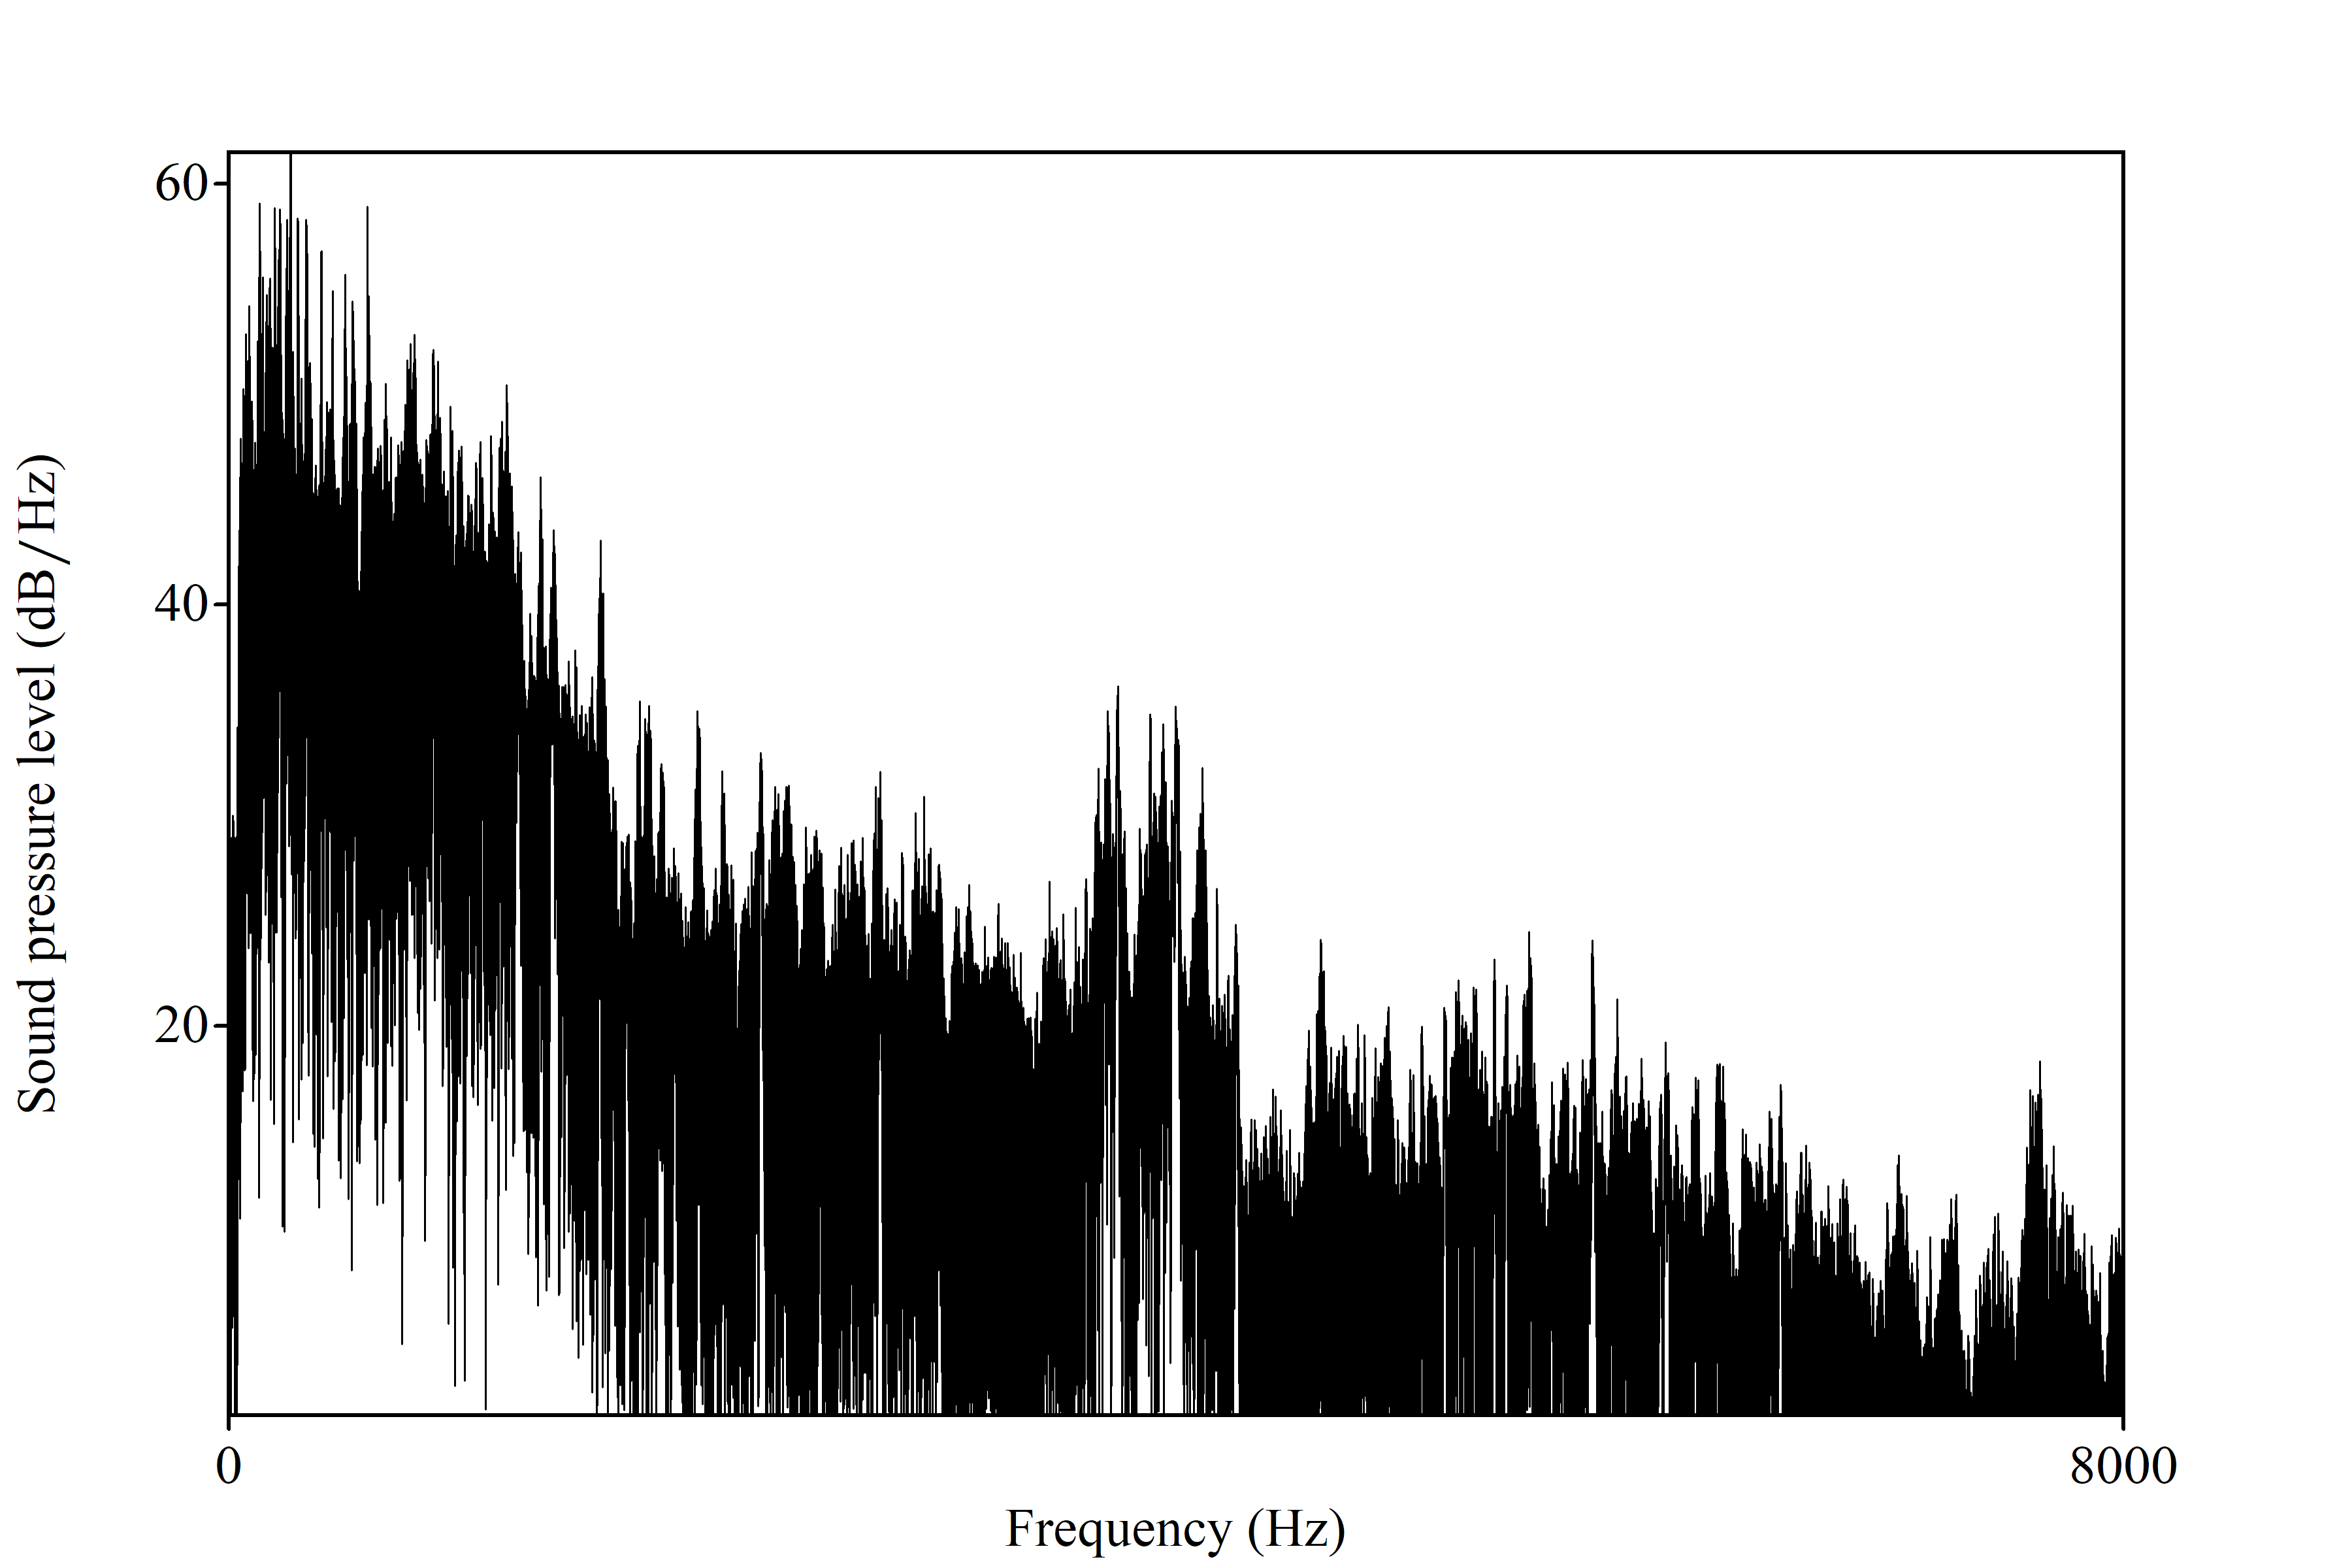
\includegraphics[width=\linewidth]{figures/ae_loss/fft_original_yee}
  \caption{original humming}
  \endminipage\hfill
  \minipage{0.5\textwidth}
  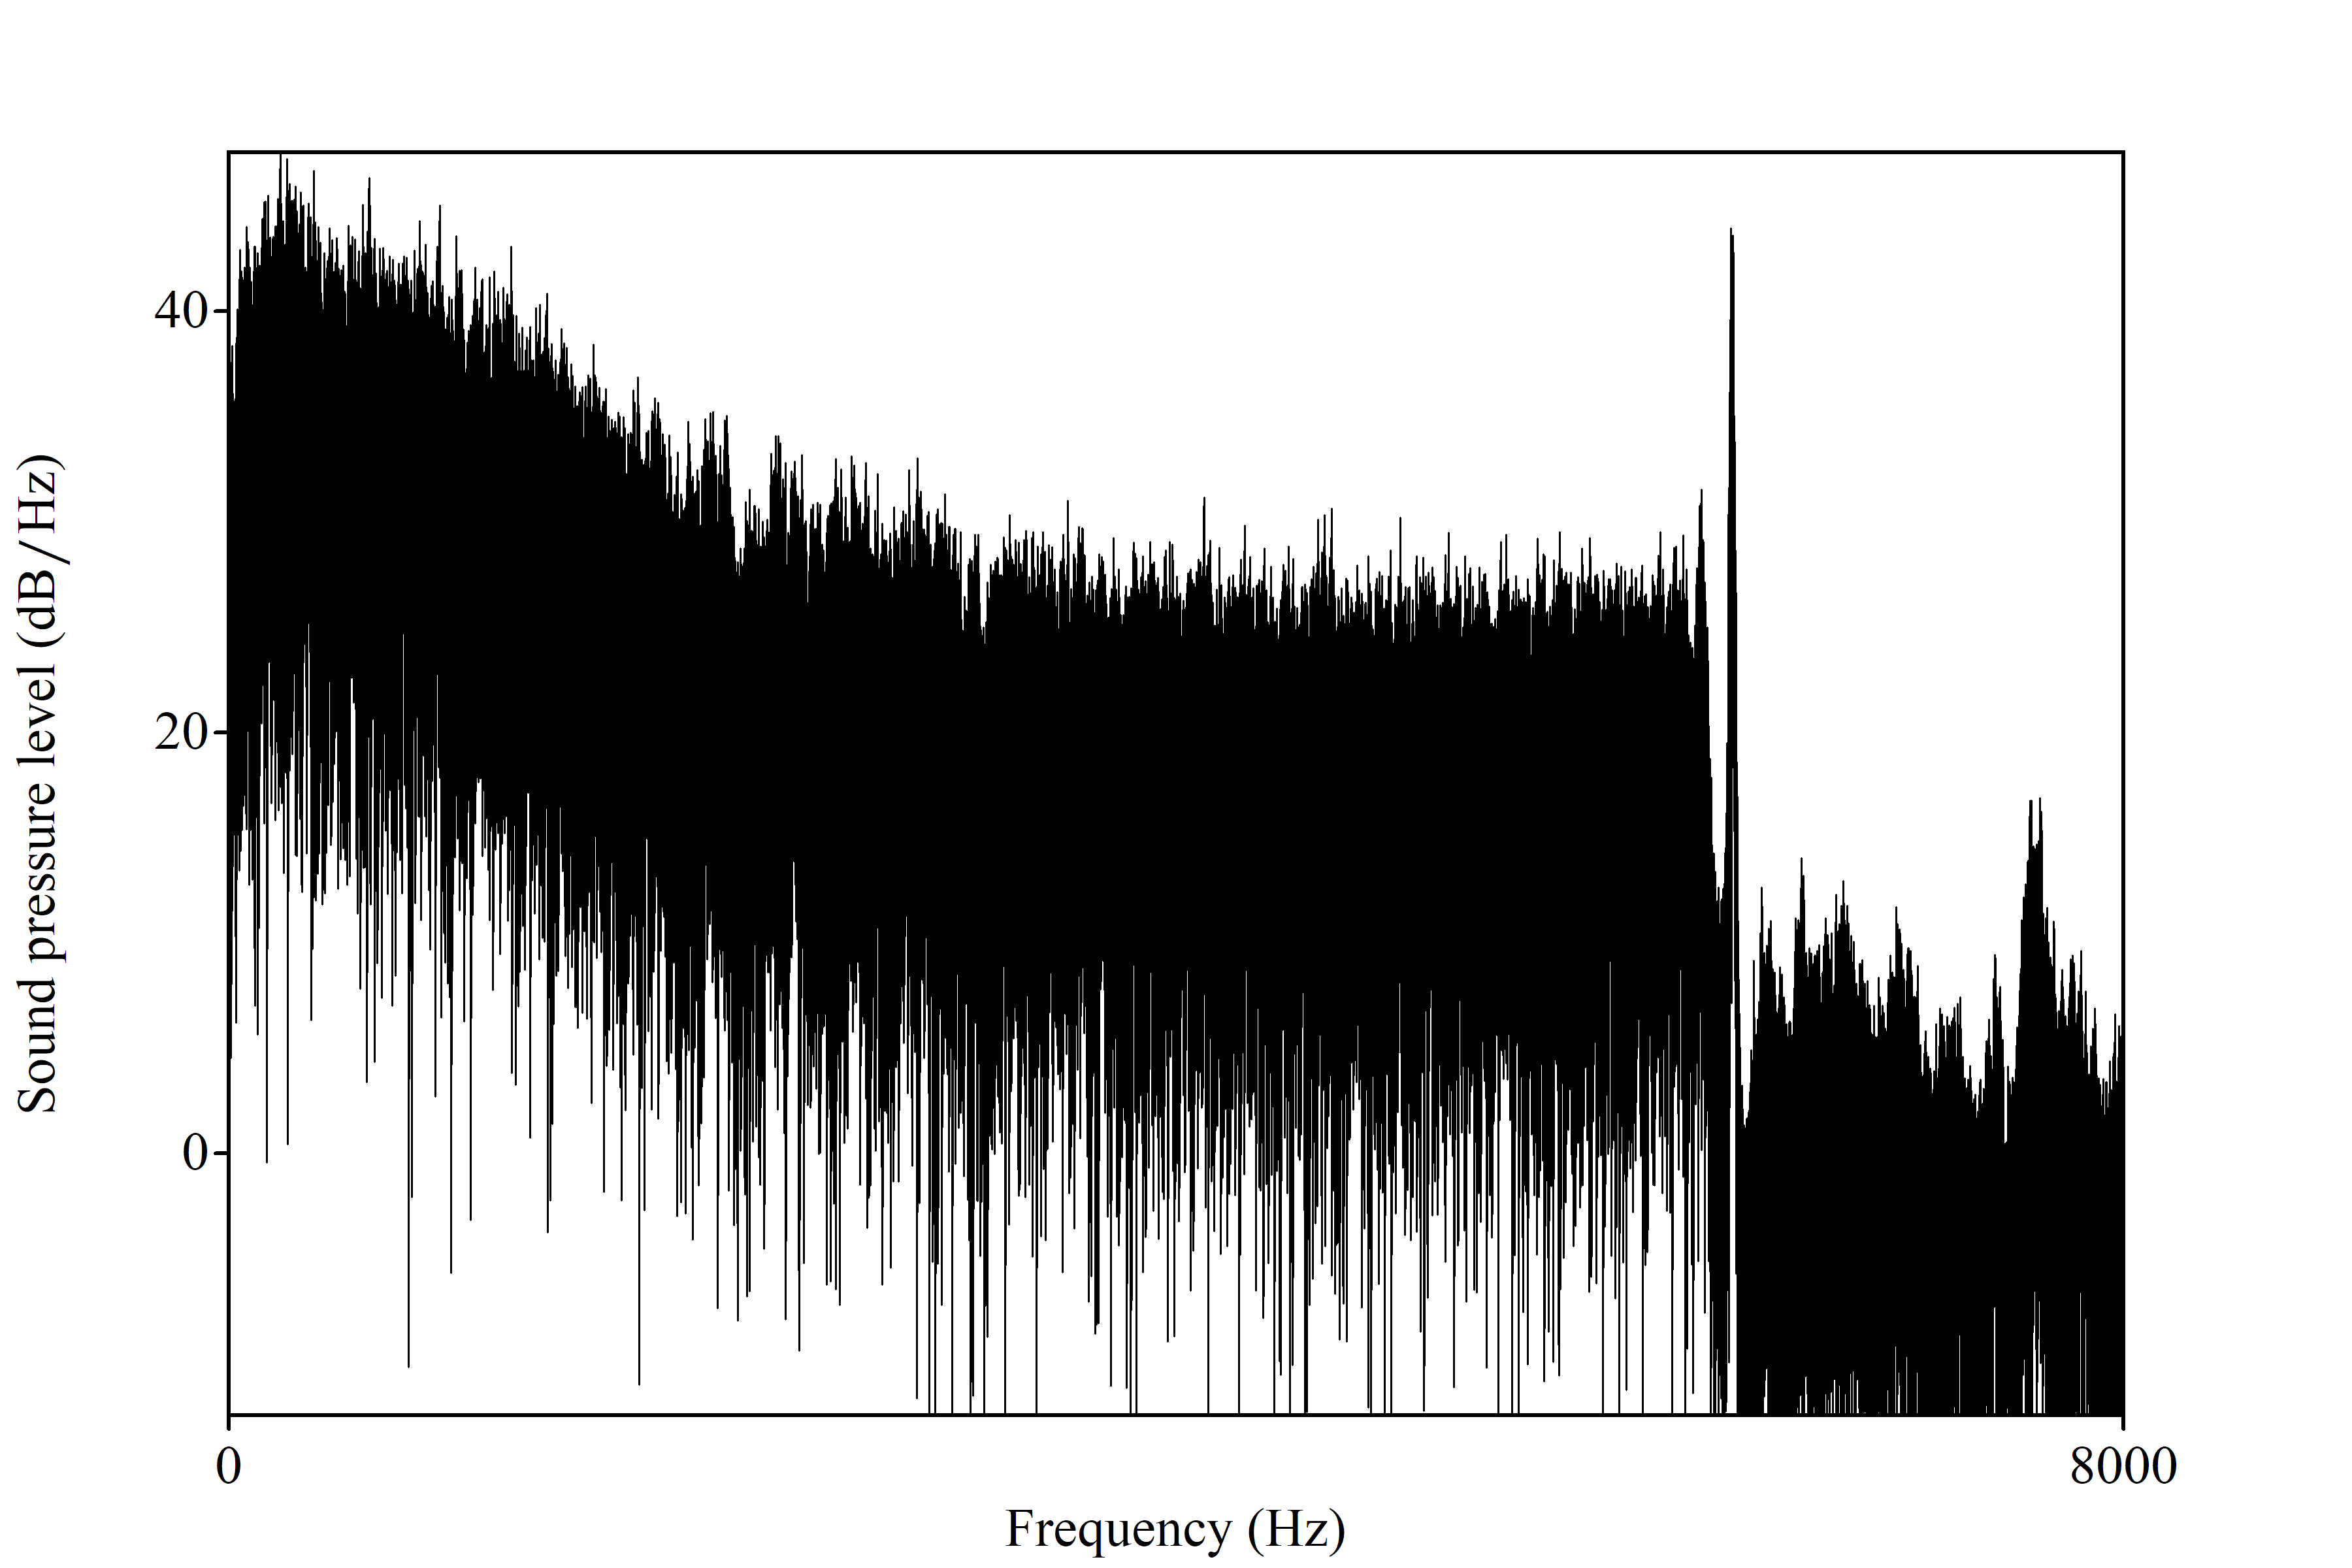
\includegraphics[width=\linewidth]{figures/ae_loss/fft_reconstruct_yee}
  \caption{reconstructed humming}
  \endminipage\hfill
\end{figure}


If you look at the result of FFT(figure 6,7), amplitude suddelny drops at the cropped boundary. This means that the model can't discriminate zero values and non-zero values. Also, there is a problem with normalization cropping and reconstructing.

\subsection{Entire model} 

\begin{figure}[!htb]
  \minipage{0.5\textwidth}
  \includegraphics[width=\linewidth]{figures/ae_target_gan_loss/spectro_original_jfla}
  \caption{original singing}
  \endminipage\hfill
  \minipage{0.5\textwidth}
  \includegraphics[width=\linewidth]{figures/ae_target_gan_loss/spectro_reconstruct_jfla}
  \caption{reconstructed singing}
  \endminipage\hfill
\end{figure}


Figure 8, 9 shows that the conversion didn't work properly. But compared to 1), reconstruction worked well, but here again, There is no emphasis, only filled with mean value.

\begin{figure}[!htb]
  \minipage{0.5\textwidth}
  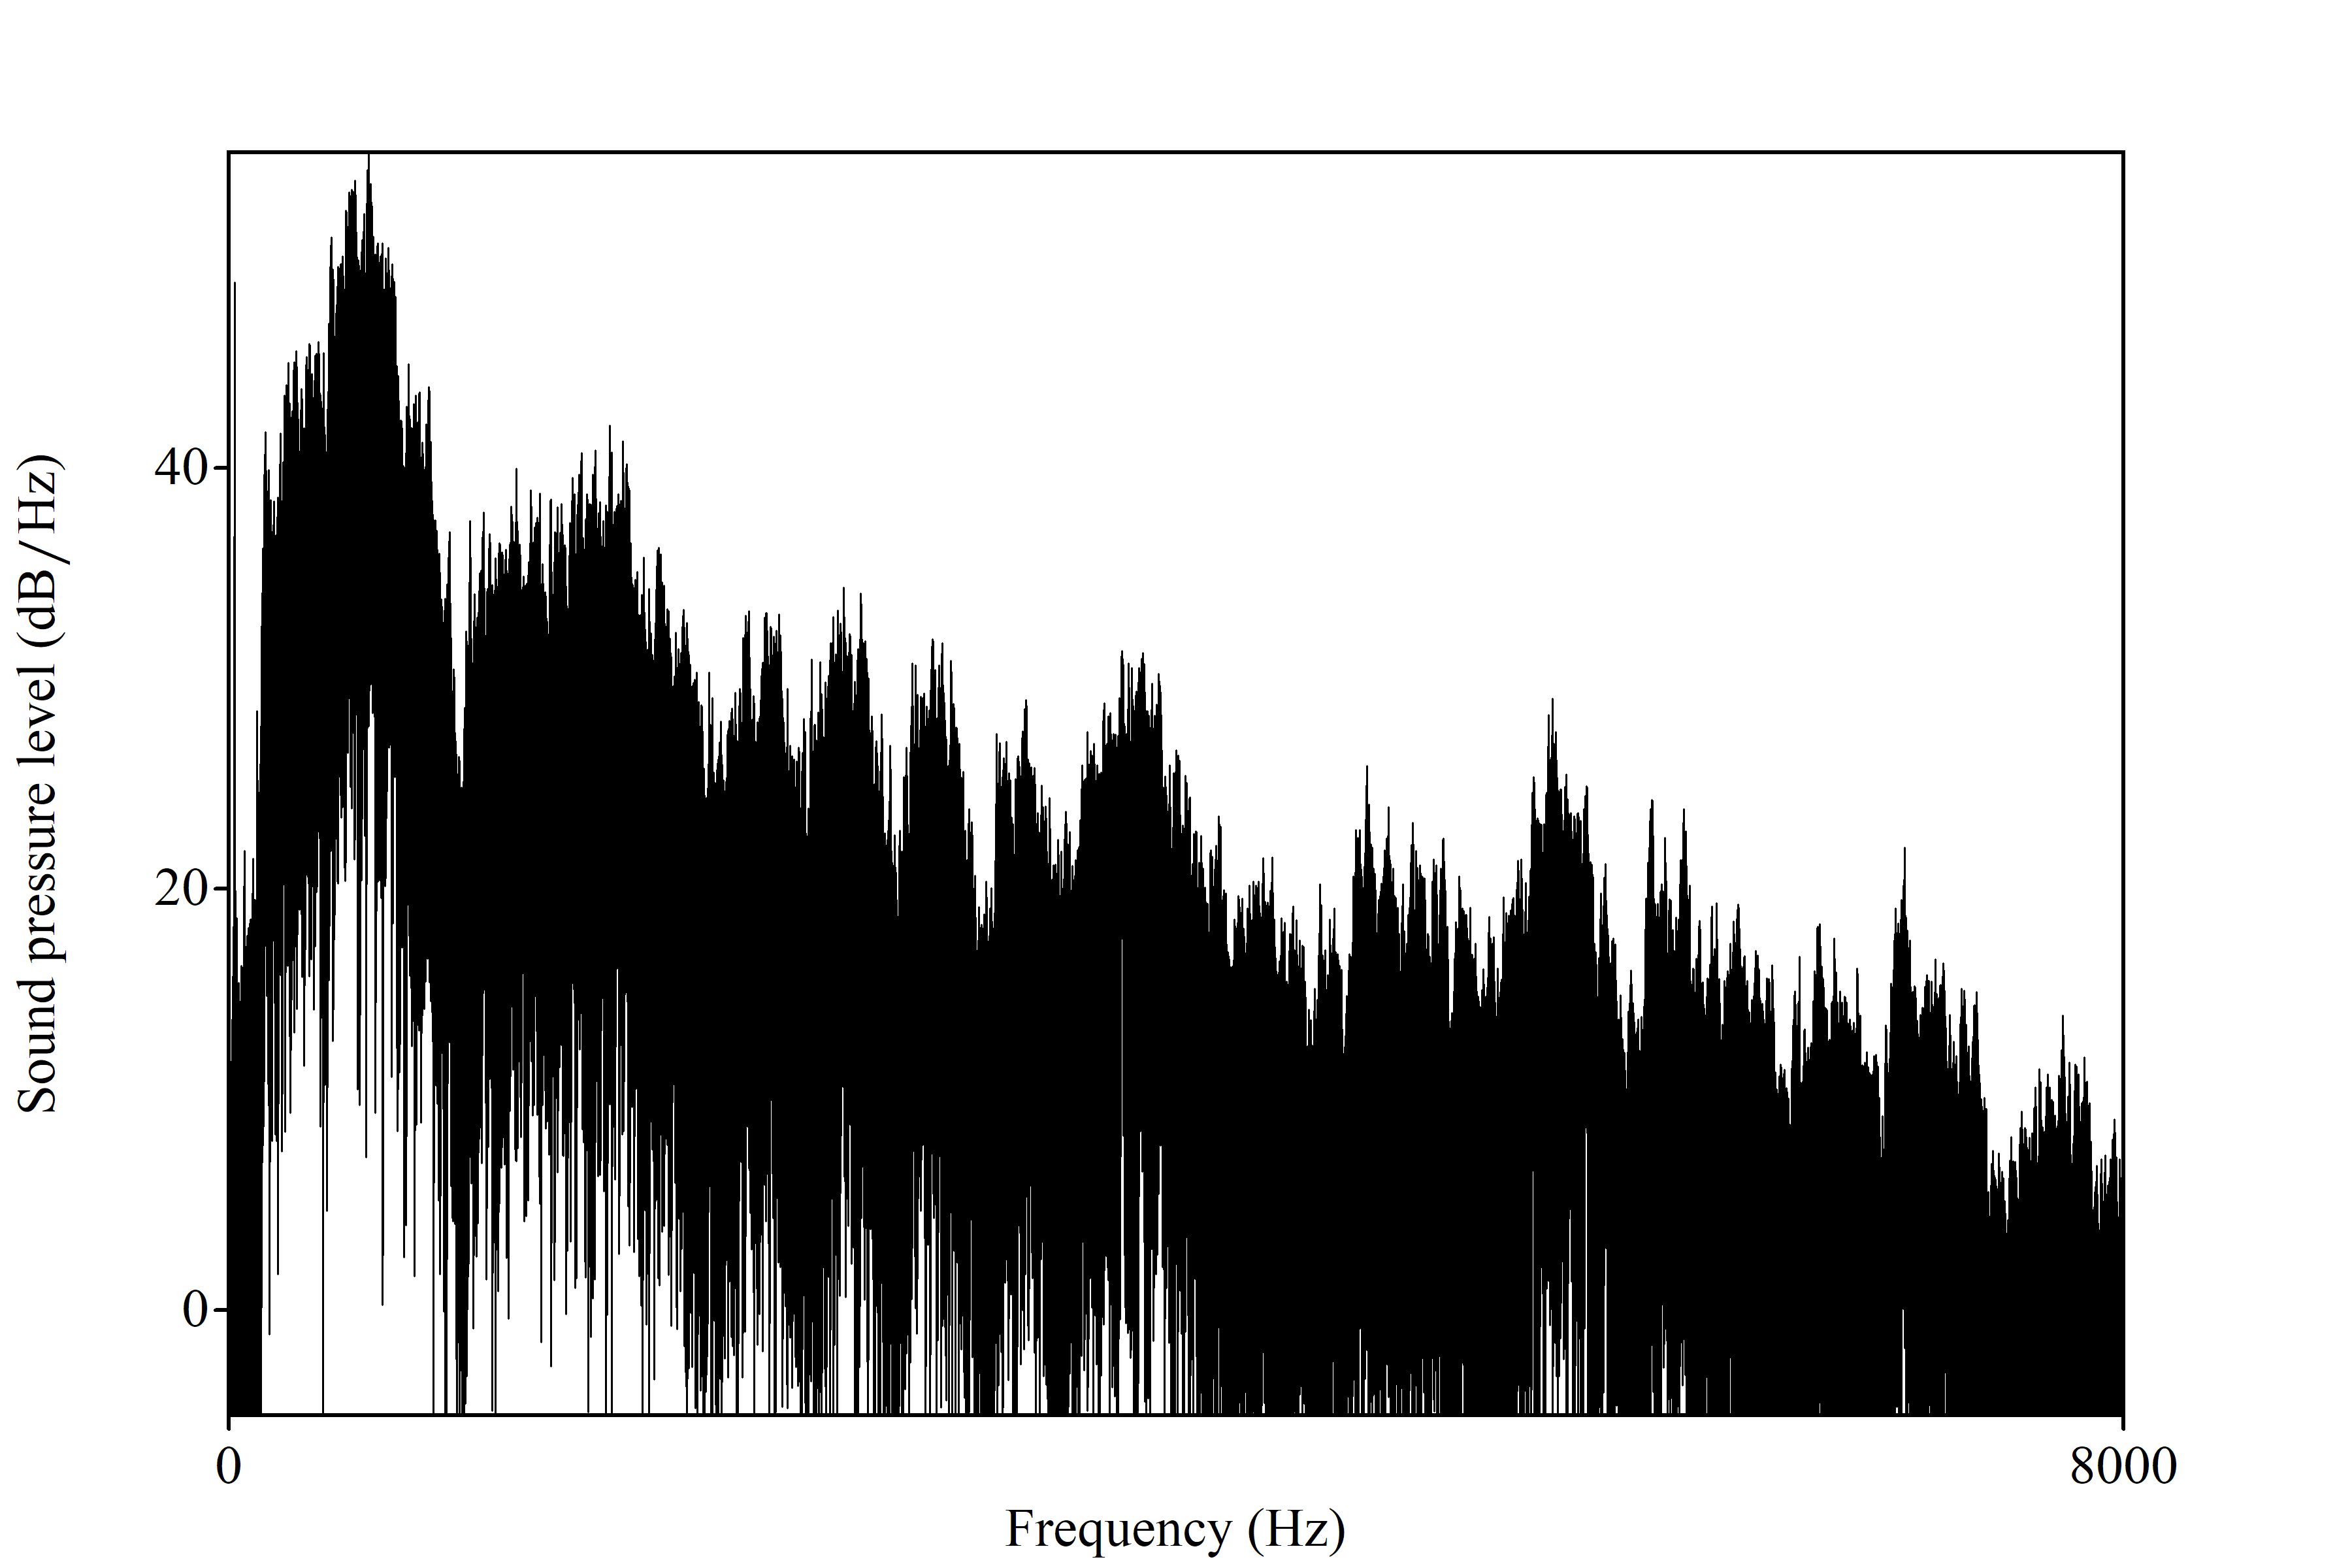
\includegraphics[width=\linewidth]{figures/ae_target_gan_loss/fft_original_speech}
  \caption{original speech}
  \endminipage\hfill
  \minipage{0.5\textwidth}
  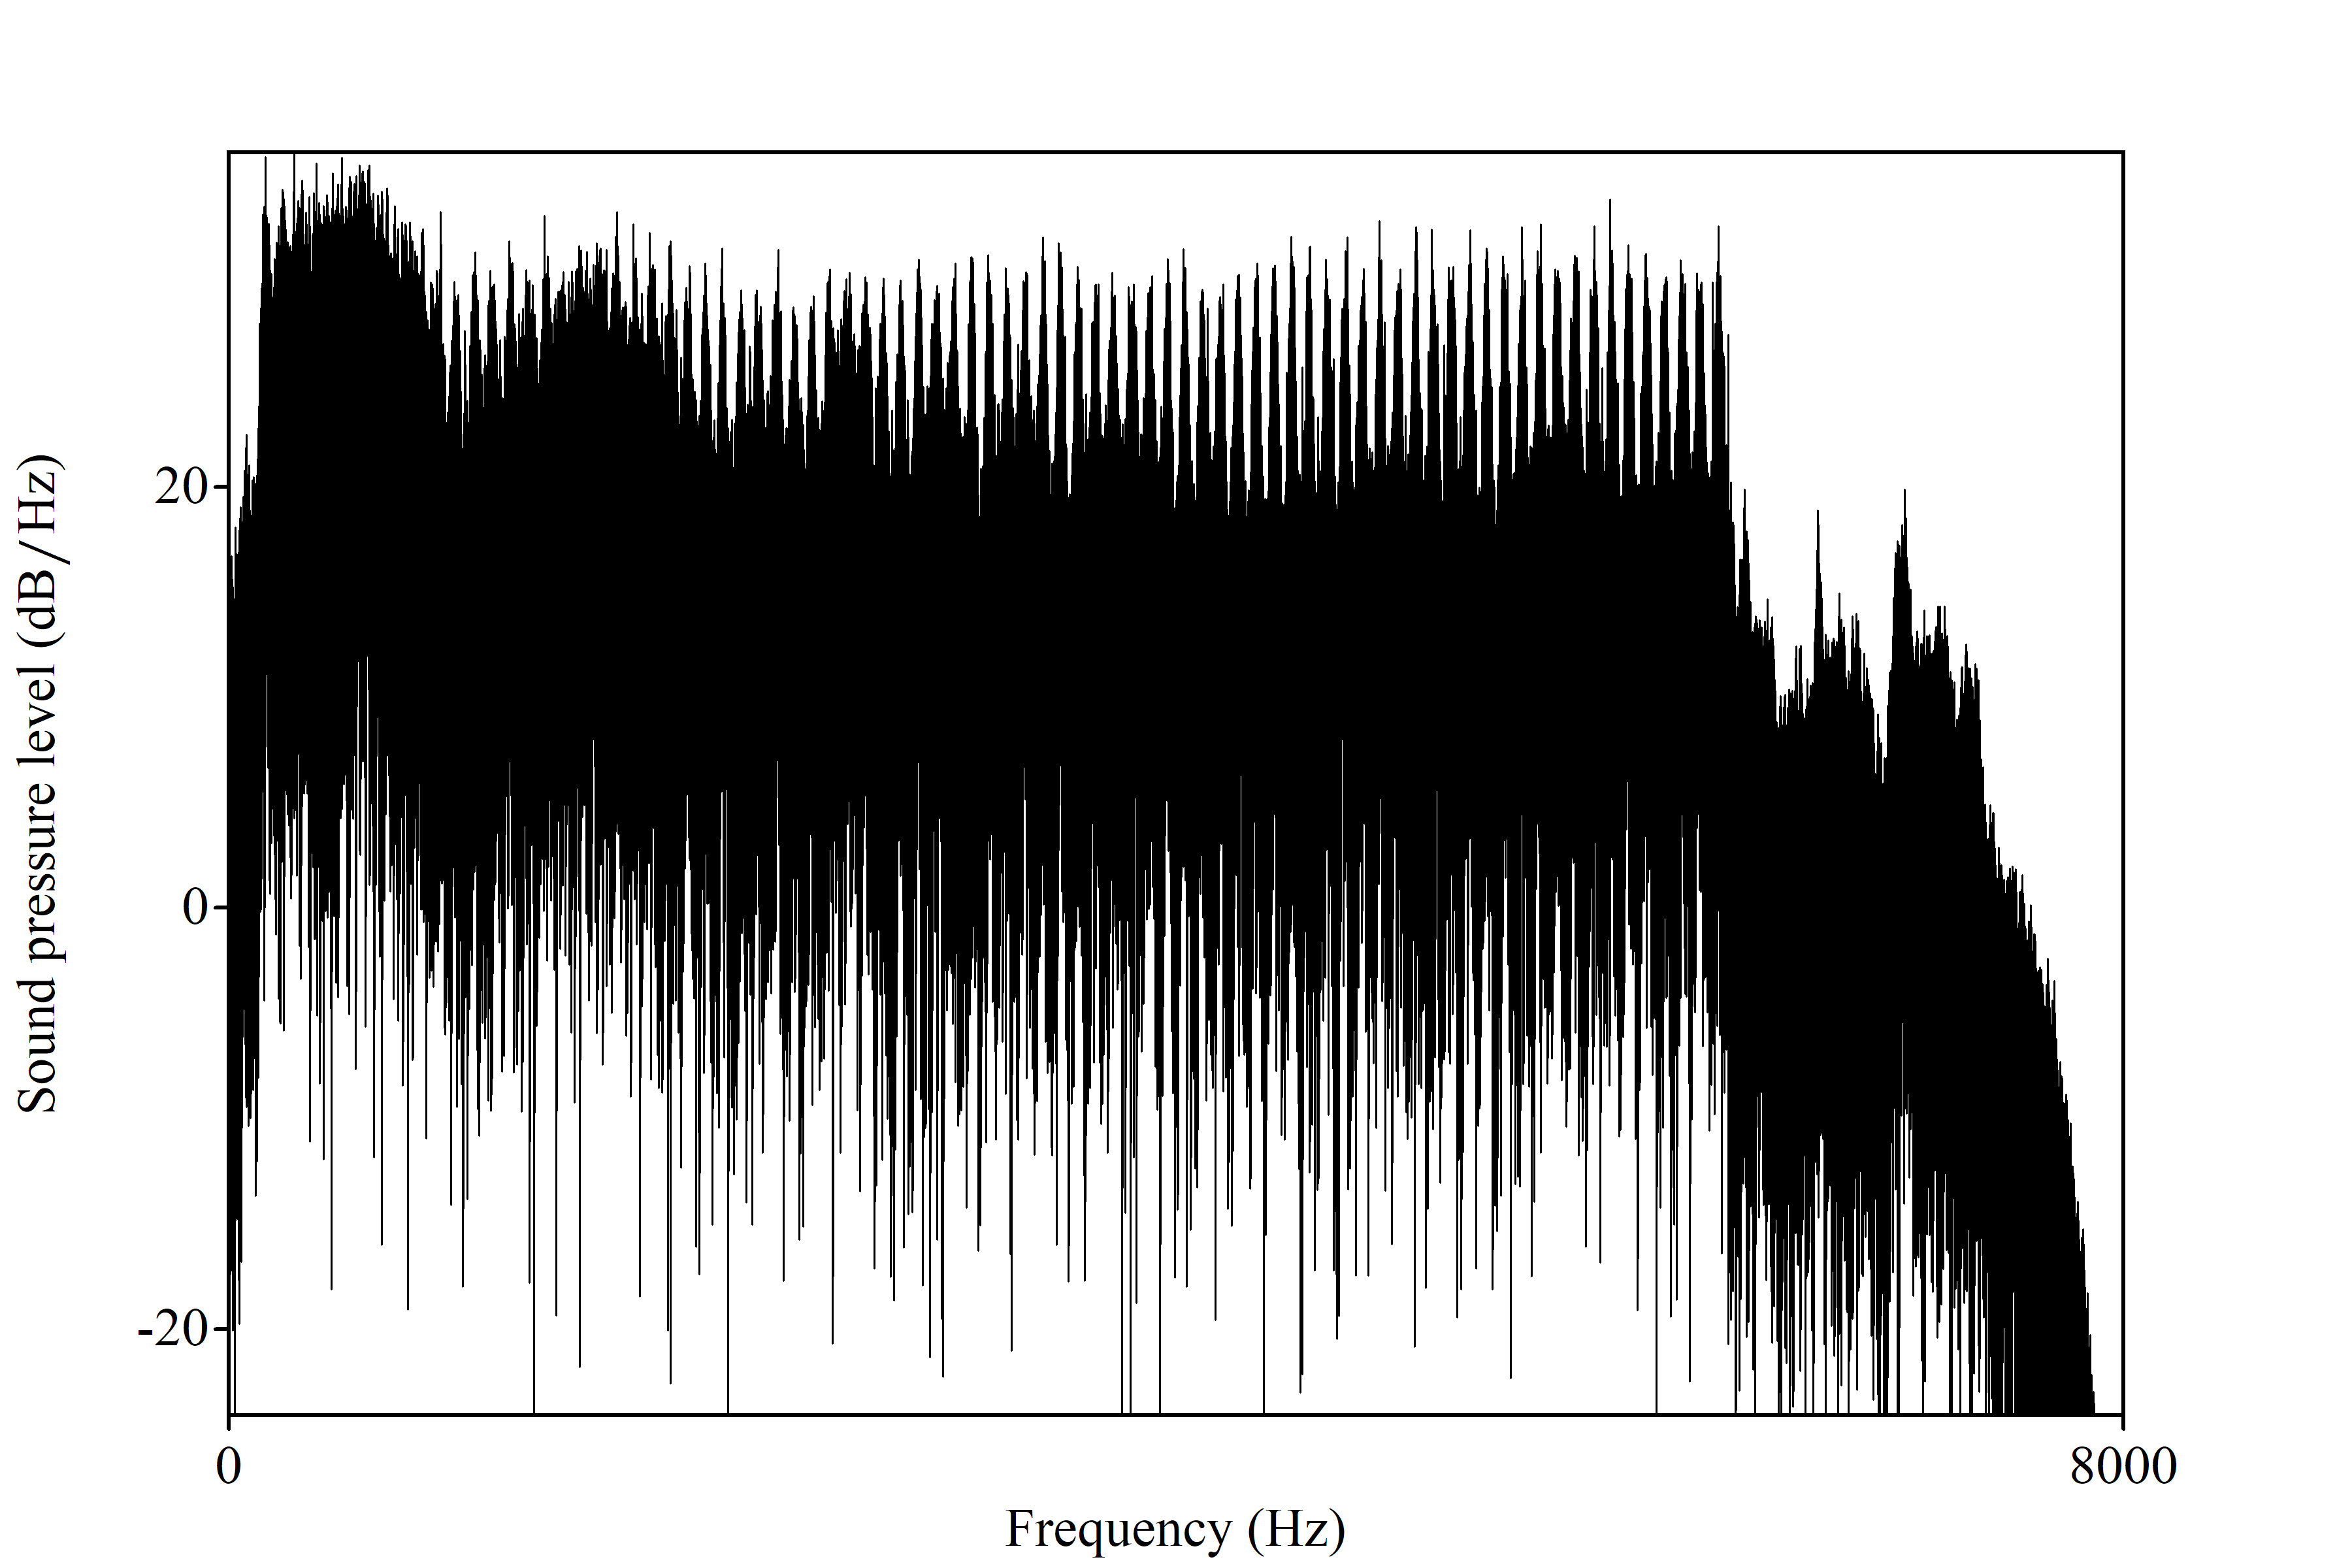
\includegraphics[width=\linewidth]{figures/ae_target_gan_loss/fft_reconstruct_speech}
  \caption{reconstructed speech}
  \endminipage\hfill
\end{figure}


Figure 10, 11 shows that the noise ratio is smaller compared to 1).

\section{Future Work}

First, we need to build more efficient structure. To reduce noise, we have to put the whole spectrogram, not the cropped one. But in this case the resolution of a spectrogram becomes too high to process it fast enough. we need to build efficient model to handle this problem.

Second, current autoencoder makes latent vector similar as a activation map in CNN. This is kind of a problem because the spectrogram now has spatial information, which may hinders the generator from generating Trump's voice. We need to add more fully connected layer to generate proper latent vector.

Third, discriminator is doing multi-task learning. We think we can apply this to autoencoder to have autoencoder extract voice features much more accurately.

Also, we have to find a way to reduce the audio reconstruction time. Current bottleneck is the conversion of spectrogram into audio. This is because Griffin-Lim algorithm is iterative. We can instead use Fast Griffin-Lim algorithm to deal with this problem. Short conversion time is very important in real-time voice conversion application and user experience.

Our model can be developed into many-to-many conversion. If our generator can generate arbitrary target voice, this is possible to convert arbitrary voice to arbitrary voice.



{\small{}\bibliographystyle{unsrt}
\bibliography{example}
}{\small \par}

\begin{comment}
{\small{}{[}1{]} Alexander, J.A.\ \& Mozer, M.C.\ (1995) Template-based
algorithms for connectionist rule extraction. In G.\ Tesauro, D.S.\ Touretzky
and T.K.\ Leen (eds.), }\textit{\small{}Advances in Neural Information
Processing Systems 7}{\small{}, pp.\ 609–616. Cambridge, MA: MIT
Press.}{\small \par}

{\small{}{[}2{]} Bower, J.M.\ \& Beeman, D.\ (1995) }\textit{\small{}The
Book of GENESIS: Exploring Realistic Neural Models with the GEneral
NEural SImulation System.}{\small{} New York: TELOS/Springer–Verlag.}{\small \par}

{\small{}{[}3{]} Hasselmo, M.E., Schnell, E.\ \& Barkai, E.\ (1995)
Dynamics of learning and recall at excitatory recurrent synapses and
cholinergic modulation in rat hippocampal region CA3. }\textit{\small{}Journal
of Neuroscience}{\small{} }\textbf{\small{}15}{\small{}(7):5249-5262.}{\small \par}
\end{comment}

\end{document}
